\documentclass[review]{elsarticle}

\makeatletter
\def\@author#1{\g@addto@macro\elsauthors{\normalsize%
    \def\baselinestretch{1}%
    \upshape\authorsep#1\unskip\textsuperscript{%
      \ifx\@fnmark\@empty\else\unskip\sep\@fnmark\let\sep=,\fi
      \ifx\@corref\@empty\else\unskip\sep\@corref\let\sep=,\fi
      }%
    \def\authorsep{\unskip,\space}%
    \global\let\@fnmark\@empty
    \global\let\@corref\@empty  %% Added
    \global\let\sep\@empty}%
    \@eadauthor={#1}
}
\makeatother

\usepackage{lineno}
\usepackage{color}
\usepackage[hidelinks]{hyperref}
\usepackage{graphicx}
\usepackage{epstopdf}
\usepackage{multirow}
\usepackage{lineno}
\usepackage{amssymb}
\graphicspath{ {./figures/} }



\modulolinenumbers[5]
\journal{Journal of \LaTeX\ Templates}

%%%%%%%%%%%%%%%%%%%%%%%
%% Elsevier bibliography styles
%%%%%%%%%%%%%%%%%%%%%%%
%% To change the style, put a % in front of the second line of the current style and
%% remove the % from the second line of the style you would like to use.
%%%%%%%%%%%%%%%%%%%%%%%

%% Numbered
%\bibliographystyle{model1-num-names}

%% Numbered without titles
%\bibliographystyle{model1a-num-names}

%% Harvard
%\bibliographystyle{model2-names.bst}\biboptions{authoryear}

%% Vancouver numbered
%\usepackage{numcompress}\bibliographystyle{model3-num-names}

%% Vancouver name/year
%\usepackage{numcompress}\bibliographystyle{model4-names}\biboptions{authoryear}

%% APA style
%\bibliographystyle{model5-names}\biboptions{authoryear}

%% AMA style
%\usepackage{numcompress}\bibliographystyle{model6-num-names}

%% `Elsevier LaTeX' style
\bibliographystyle{elsarticle-num}
%%%%%%%%%%%%%%%%%%%%%%%

\begin{document}

\begin{frontmatter}

\title{Barreling formation during the axial compressive experiments on cubic
samples with orthotropic properties {\color{red} Preliminary title}}
%%\tnotetext[mytitlenote]{Fully documented templates are available in the
% elsarticle package on \href{http://www.ctan.org/tex-archive/macros/latex/contrib/elsarticle}{CTAN}.}

%% Group authors per affiliation:






%%\fntext[fn1]{This is the specimen author footnote.}
%%\fntext[fn2]{Another author footnote, but a little more longer.}
%%\fntext[fn3]{Yet another author footnote. Indeed, you can have any number of
% author footnotes.}

\author{Alexey Vorobyev\corref{cor1}}
\ead{alexey.vorobyev@angstrom.uu.se}

\cortext[cor1]{Corresponding author}

\author{Nico P. van Dijk}
\author{Kristofer Gamstedt}

\address{Uppsala University, Division of Appplied Mechanics,
Uppsala, Sweden }



\begin{abstract}
This template helps you to create a properly formatted \LaTeX\ manuscript.
\end{abstract}

\begin{keyword}
\texttt{elsarticle.cls}\sep \LaTeX\sep Elsevier \sep template
\MSC[2010] 00-01\sep  99-00
\end{keyword}

\end{frontmatter}

\linenumbers

\section{Introduction}
Compressive experiments are considered to be one of the most common
\color {red} method for identifying engineering constants such as Young's
modulus, Poisson's ratio and Shear modulus. General approach is to measure material response 
due to applied external load \textit{\color {red} Add the citations on
the compressive experiments methods.Give suggestions on different standards}.
The response is usually a displacement between certain points on the
observable plane of the specimen. To do that one can use strain gauges. Usually
strain gage allow to measure the mutual displacements between two points. This
is considered to be the limitation of the method\textit{\color {red} I have
to either cite it or check the best way to write it}. Another methods to measure
strains is Digital Image Correlation (DIC). This method becoming popular due to
the simplicity and possibility to measure strains on an objects with complex
geometry.


\begin{itemize}
\color{red}  



\item what problem was studied?
\item Introduction of the problem
\item Give the context of the problem
\item Reviews of previous works
\item Justification of work
\item Scopes and objectives
\item Interest the reader
\item Provide the transition to the rest
\end{itemize}

\section{Materials and Methods}
\section{Model}

The finite element program COMSOL Multiphysics 4.4 \cite{Comsol} was used for
the experimental simulations.
The entire cube (Figure \ref{fig:cubemesh})  with singular side was modeled with
3D solid elements.
The platens of universal testing machine were not considered in the model.
Instead compressive load was simulated as prescribed displacement and normally
applied to the top surface of the cube towards the lower plane. The
displacement was performed by 0.01 and 0.1 dimensional units which corresponds
to approximate 1\%  and 10\% of average strain respectively. The bottom surface
was constrained from the displacement along \textit{Z} axis. However mutually perpendicular edges of the bottom and top surfaces were aloud to move in its perpendicular directions along \textit{X} and \textit{Y} axises respectively.

A \textit{Free Quad} mesh was placed on a top surface and swept throughout
the whole geometry using \textit{Quadrilateral} meshing method which generates
hexahedrons. We have solved the model using different number of FE. The model
contained 1000 finite elements. This number was identified by solving and
refining the elements multiple times while identifying best performance vs.
accuracy of solution. 

\begin{description}
\item[{\color {red}Material input parameters}]
\end{description}
We simulated orthotropic, transverse isotropic and isotropic material behaviour.
The model was linear elastic. Material properties were experimentally determined
based on compression tests \textit{insert table with the constants}.  

\begin{description}
\item[{\color {red}Conclusions for the model}]
\end{description}

Simulations of experiments in compression are not new. Previously the
orthotropic samples were simulated by \cite{Toftegaard1999849} in order to investigate the effect of
geometrical imperfections of prism samples on identification of engineering
constants by simulating the strain field in relation to the measurements
obtained using the strain gauge. 
Present work uses DSP in order to obtain the experimental strain field, which
contains strain data of observed area and not between two points as it is for the strain gauge. 
Another simulation was performed by \cite{Chen001}.
He has simulated the behaviour of the specimen with geometrical
imperfections on a locked hemispherical seat during the compressive experiments
of thick section composite materials.





\begin{figure}[h]
\centering
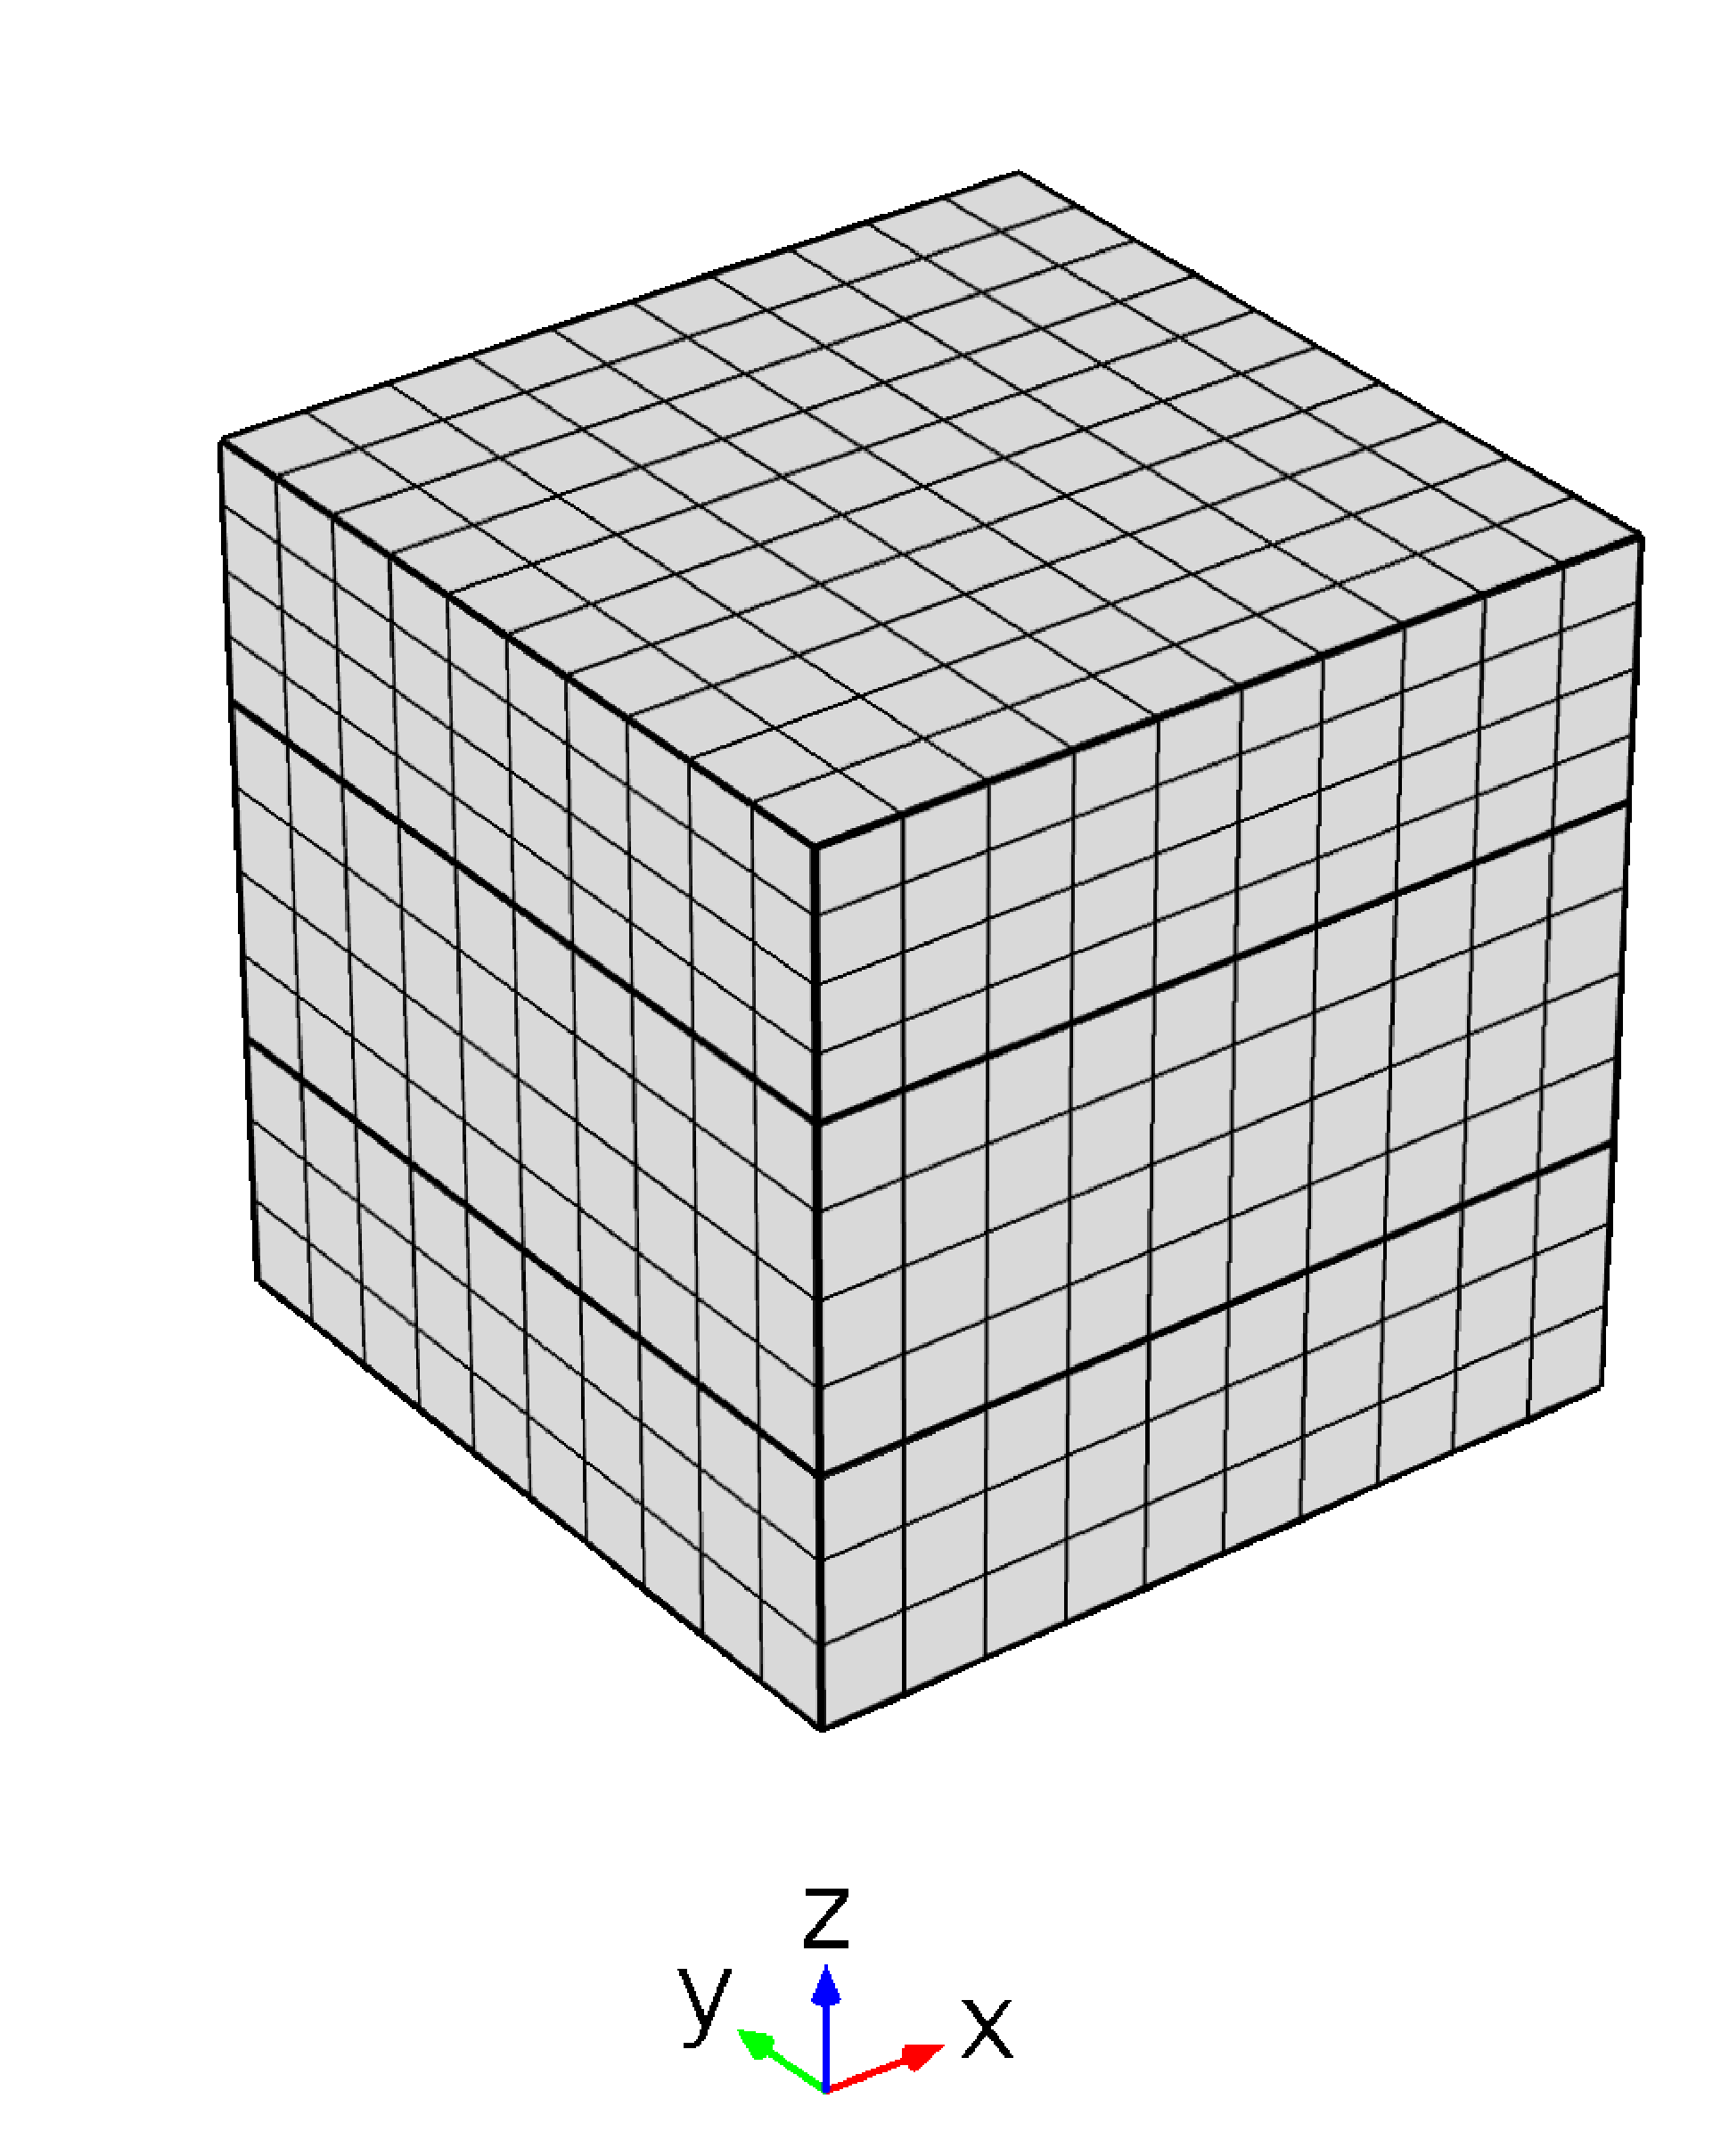
\includegraphics[width=5cm]{CubeFEM.eps}
\label{fig:cubemesh}
\caption{\label{fig:cubemesh} Finite element model of cubic specimen}
\end{figure}


\begin{description}
\item[{\color {red}Friction}]
\end{description}

The friction between platens and specimen is consider to be a reason for the
barrelling formation \cite{Narayanasamy198821, kulkarni1969}.  To simulate that
friction we have introduced friction parameters that were applied to the mutually orthogonal
edges on the top and the bottom surface of the cube. Those parameters were
acting as a resistance for displacement varying from zero and up to the value
which equals to the stiffness along \textit{Z} axis of the cube.

\textit{\color {red}Add the picture that is showing the axises and add the
description to the the text in accordance to that. Add the bottom surface, the
free edges the friction, the coefficients, the variability of frictions that }

\begin{description}
\item[{\color {red}Obtaining strain fields both 2D and 3D}]
\end{description}

\begin{itemize}
\color{red}
\item How was the problem studied 
\item Description of FEM model, parameters, application, details of the model
\item Describe the experimental setup, materials and procedure
\end{itemize}


\section{Results and Discussions}
\begin{itemize}
\color{red}
\item What were the findings?

	\begin{enumerate}
	\color{black}
		\item Barelling formation is less in transverse isotropic and orthotropic
		material.
		\item 
	\end{enumerate}



\item Use diagrams and/or tables, objective and truthful presentation
\item Results and discussion distinguishable
\item New and old results and discussion
\end{itemize}


\section{Conclusions}

\section*{Acknowledgements}

\section*{References}


\pagebreak

\section*{Tables}

\begin{description}

\item[]
\begin{table}[ht]\
\caption{Engineering constants used in model} % title of Table
\centering % used for centering table
\begin{tabular}{l c c c c c c c c c} % centered columns (4 columns)
\hline\hline %inserts double horizontal lines
Model & $E_{1}$ (GPa) & $E_{2}$ (GPa) & $E_{3}$ (GPa) & $\nu_{12}$ & $\nu_{13}$
& $\nu_{23}$ & $G_{12}$ (GPa) & $G_{13}$ (GPa) & $G_{23}$ (GPa) \\ % inserts
% table heading

\hline % inserts single horizontal line
Orthotropic & 1.49 & 0.89 & 12.14 & 0.66 & 0.06 & 0.04 & 0.2 & 0.6 & 0.72 \\
% inserting body of the table
Transverse isotropic & 1.49 & $E_1=E_2$ & 12.14 & 0.66 & 0.06 & 0.04 & 0.2 &
 0.6 & 0.72\\
Isotropic & - & - & 12.14 \\
 [1ex] % [1ex] adds vertical space
\hline %inserts single line
\end{tabular}
\label{table:nonlin} % is used to refer this table in the text
\end{table}

\it{\color{red}Check whether i need to add the isotropic parameters and transv
ortho}

\end{description}

%%%%%%%%%%% VIDEO CAPTIONS

%% If submitting video's as a supplement to the manuscript, include only the video captions here (not the figures).  Videos are uploaded separately in the online Elsevier Editorial Submission process.  If videos are not included, comment out this section.

%% Do not remove the page break here.
\pagebreak

\bibliography{mybibfile}

\end{document}